\section{Model Training}
\label{sec:training}

\subsection{Preprocessing and Pipelines}
Every configuration is a single \texttt{imbalanced-learn} pipeline,
and its preprocessing stage has two channels. Trees receive nominal
attributes through an \texttt{OrdinalEncoder}, whose arbitrary
integer order constrains the value groupings a tree can form, while
numeric attributes pass through unscaled. LR and SVC instead receive
\texttt{OneHotEncoder} output with \texttt{handle\_unknown='ignore'}
plus \texttt{StandardScaler} on the numerics. Every fit-type step,
namely imputation, encoding, scaling and SMOTE where applicable,
lives inside the pipeline: parameters are fitted on the training fold
only, and the validation fold is merely transformed, as
Figure~\ref{fig:pipelines} shows. On sick the two fully missing TBG
columns are dropped outside the pipeline, and the remaining gaps are
imputed in-fold, numerics by the training-fold mean and nominals by
the training-fold mode. Credit-g needs no cleaning at all, as it has
zero missing values and zero duplicate rows.

\begin{figure}[H]\centering
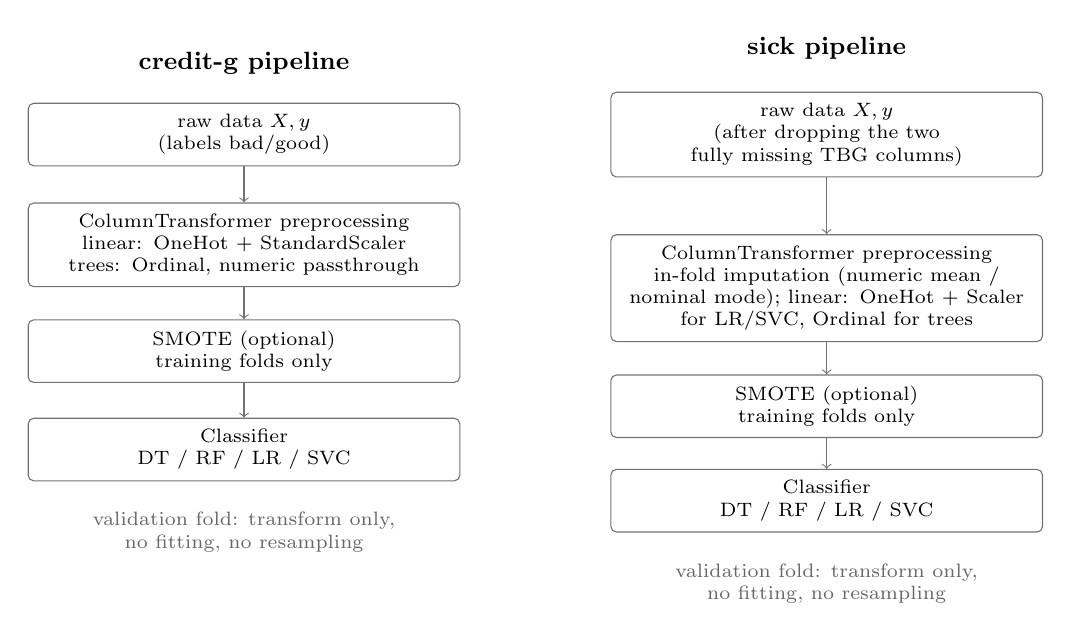
\begin{tikzpicture}[
  box/.style={draw=black!55, rounded corners=2pt, align=center,
              font=\scriptsize, text width=5.2cm, inner sep=4pt},
  ttl/.style={font=\small\bfseries},
  note/.style={font=\scriptsize, text=black!60, align=center}]
% ---- credit-g column ----
\node[ttl]        at (0,0.9)    {credit-g pipeline};
\node[box] (raw1) at (0,0)      {raw data $X,y$\\(labels bad/good)};
\node[box] (pre1) at (0,-1.4)   {ColumnTransformer preprocessing\\linear: OneHot + StandardScaler\\trees: Ordinal, numeric passthrough};
\node[box] (sm1)  at (0,-2.75)  {SMOTE (optional)\\training folds only};
\node[box] (clf1) at (0,-4.0)   {Classifier\\DT / RF / LR / SVC};
\draw[->,black!55] (raw1) -- (pre1);
\draw[->,black!55] (pre1) -- (sm1);
\draw[->,black!55] (sm1) -- (clf1);
\node[note]        at (0,-5.05) {validation fold: transform only,\\no fitting, no resampling};
% ---- sick column ----
\node[ttl]        at (7.4,1.1)  {sick pipeline};
\node[box] (raw2) at (7.4,0)    {raw data $X,y$\\(after dropping the two\\fully missing TBG columns)};
\node[box] (pre2) at (7.4,-1.95) {ColumnTransformer preprocessing\\in-fold imputation (numeric mean /\\nominal mode); linear: OneHot + Scaler\\for LR/SVC, Ordinal for trees};
\node[box] (sm2)  at (7.4,-3.45) {SMOTE (optional)\\training folds only};
\node[box] (clf2) at (7.4,-4.65) {Classifier\\DT / RF / LR / SVC};
\draw[->,black!55] (raw2) -- (pre2);
\draw[->,black!55] (pre2) -- (sm2);
\draw[->,black!55] (sm2) -- (clf2);
\node[note]        at (7.4,-5.7) {validation fold: transform only,\\no fitting, no resampling};
\end{tikzpicture}
\caption{The two dataset-specific pipelines share one three-stage
structure, from preprocessing through optional SMOTE to the
classifier. They differ only inside the preprocessing stage, where
sick additionally imputes missing values in-fold. The validation fold
is only transformed, never fitted or resampled.}
\label{fig:pipelines}
\end{figure}

\subsection{Locked Configuration}
All hyperparameters were frozen once, before any evaluation, with
\texttt{random\_state=42} on every stochastic component:
\begin{itemize}
\item DT: \texttt{criterion='entropy'}, $\alpha_{\text{ccp}}=0.01$;
\item RF: $n_{\text{estimators}}=100$;
\item LR: \textit{max\_iter}=1000, leaving convergence headroom on
the 60--80 one-hot dimensions;
\item SVC: RBF kernel, $C=1.0$, \texttt{probability=True}.
\end{itemize}
The values follow library defaults or simple round settings and were
deliberately not tuned, so no evaluation signal could leak into model
selection. Together with the locked splits and the seed they make the
pipeline reproducible. Reported numbers are checked against the
archived outputs within a tight tolerance, since floating-point
results can still differ slightly across hardware and threading
configurations.
% TODO(E): cite scikit-learn (Pedregosa et al., 2011) and
% imbalanced-learn (Lemaitre et al., 2017) once bib keys are fixed.

\subsection{Evaluation Protocol}
Two fixed protocols are used. The first is stratified 10-fold
cross-validation with \texttt{shuffle=True} and
\texttt{random\_state=42} over the full data, reported as
mean$\pm$std over folds with $ddof=0$. The second is a one-off 70:30
stratified holdout, 700/300 on credit-g and 2640/1132 on sick,
evaluated exactly once per locked configuration. Since the champion
configuration was selected on the full-data CV and those folds
overlap the holdout rows, the holdout is not an untouched final test.
We therefore report the two protocols as fixed internal evaluations
and note the selection overlap as a limitation. The minority class is
the positive class throughout, bad on credit-g and sick on sick. All
metrics come from one shared evaluation module: accuracy,
positive-class precision, recall and F1, ROC-AUC, Cohen's $\kappa$,
balanced accuracy, macro-F1, and the credit-g cost
$(5\,\mathit{FN}+\mathit{FP})/N$.

% [review note] Former subsection "Dataset-Specific Differences" (table
% tab:pipeline-diff) deleted after review: the differences it tabulated are
% already given in Sections 3a/3b and in the pipeline figure above.

% [M6, per D's v2.1 write-back note] The former "Ensemble study setup" paragraph
% now lives at the start of Section 6.5 (sec6_results.tex) and was removed here.
